\documentclass[parskip=full, numbers=noenddot]{scrreprt}

\usepackage[english]{babel}
\usepackage[utf8]{inputenc}
\usepackage{csquotes}
\usepackage[backend=biber, doi=false, isbn=false, url=false, date=year]{biblatex}
\addbibresource{mainreport.bib}

\usepackage{graphicx}
  \graphicspath{ {./graphics/} }
\usepackage{url}
\usepackage{varioref}
\usepackage{tabularx}
  \newcolumntype{L}{>{\raggedright\arraybackslash}X}
  \usepackage[version=4]{mhchem}
\usepackage{siunitx}
\usepackage{booktabs}
\usepackage{longtable}


\author{Arin Wongprommoon\thanks{\texttt{aw729@cam.ac.uk}} \\University of Cambridge}
\title{Optimising production of citramalate based on the \emph{E. coli} kinetic and stoichiometric models}
\subtitle{Project report}
\date{17 August 2018}

\begin{document}

\maketitle

\tableofcontents

\begin{abstract}
  Using living organisms to synthesise chemicals is an alternative to synthesising chemicals from fossil fuels, as it serves as a renewable resource with potentially high efficiency and low cost. The procedures can be sped up by optimising conditions using mathematical models. Citramalate ((2\emph{S})-2-hydroxy-2-methylbutanedioate) is a chemical of industrial interest as it can be a precursor for methacrylic acid, a monomer for the production of plastics. 
  
  This project used modelling approaches to find conditions that maximise the production of citramalate. The kinetic model described by Millard \emph{et al.}~\cite{millard_metabolic_2017} and the stoichiometric model described by Orth \emph{et al.}~\cite{orth_comprehensive_2011}, both for \emph{E. coli} metabolism, were extended by adding a reaction that produced citramalate from acetyl coenzyme A and pyruvate. \emph{E. coli} was chosen as the model organism as its metabolism is very well characterised in the literature. The project employed Python and libraries specific to genetic algorithms, modelling, and manipulating information presented in SBML (systems biology markup language).
  
  First, the effect of $V_{max}$ values of reactions in the kinetic model on productivity of citramalate was investigated. This parameter was chosen as it can be easily tested \emph{in vivo} by relying on the principle that $V_{max}$ is proportional to enzyme concentration. The differential evolution genetic algorthim was then employed to compute the set of $V_{max}$ values of reactions that optimises the production of citramalate, assuming Michaelis-Menten kinetics. In the second part of the project, information from the kinetic model was used to enrich the stoichiometric model. The possible values of fluxes through each reaction were used to set the bounds for each reaction in the stoichiometric model. Flux balance analysis (FBA) was then performed to evaluate the highest possible flux through the citramalate-producing reaction as a proxy for citramalate productivity. Finally, composition of the Lund medium~\cite{eastham_process_2015} was studied in an attempt to create bounds for relevant uptake reactions.
  
  The project took place at the Cambridge Systems Biology Centre, Department of Biochemistry, in Prof Steve Oliver's group. Research associate Dr Jorge J\'ulvez supervised me throughout the project. The project was entirely computational, and ran from 25 June 2018 to 17 August 2018.
\end{abstract}

\chapter*{Introduction}
\label{ch:intro}

The project concerns two models of \emph{E. coli} metabolism: a kinetic model described by Millard \emph{et al.} in 2017~\cite{millard_metabolic_2017} and a stoichiometric model described by Orth \emph{et al} in 2011~\cite{orth_comprehensive_2011}. The kinetic model concerns a smaller set of reactions, but it contains initial conditions -- substrate concentrations and flux through reactions -- which the stoichiometric model lacks.

The kinetic model contains 68 reactions, 49 of which include $V_{max}$ as a parameter (see appendix~\ref{ap:kineticreactionlist}). Of these, 41 correspond to real enzyme-catalysed reactions. To investigate citramalate production, a 69th reaction called CITRA\_SYN was added to the model. It models the reaction:

\begin{center}
  acetyl-CoA + pyruvate + \ce{H2O} $\rightarrow$ CoA-SH + \ce{H^+} + citramalate
\end{center}

with the Michaelis-Menten kinetic law

\[
  \frac{\mathrm{d}[citramalate]}{\mathrm{d}t} = 
  \frac{V_{max} \cdot [acetyl-CoA]}{[acetyl-CoA] + K_{m}}
\]

which assumes that pyruvate is saturating. $V_{max}$ is set to 4 mM s\textsuperscript{-1} and $K_{m}$ to 0.495 mM in the modified model.

Citramalate productivity is defined as $\mu \cdot Y_{P/S}$, where $\mu$ is the growth rate in reciprocal time units (h\textsuperscript{-1} in this project) and $Y_{P/S}$ is defined as the mass of the product (citramalate) divided by the mass of the substrate (glucose). Manipulating the SBML file required the Python library \texttt{libsbml} and running simulations employed the \texttt{roadrunner} module. The simulations were from 0 to 7,200 seconds, at which steady-state was attained for almost all conditions. Verification of steady-state conditions is discussed in subsection~\ref{ssec:steadystate}.

The stoichiometric model contains 2,584 reactions, and I mapped 57 to their equivalents in the kinetic model (detailed in section~\ref{sec:mapping}). By default, most of these reactions are unbounded as stated in the materials and methods section of Orth \emph{et al.} (2011)~\cite{orth_comprehensive_2011}. In a similar vein to the kinetic model, a 2,585th reaction for citramalate production was added to the stoichiometric model using the \texttt{cobra} module in Python. In addition to the citramalate synthesis reaction, a sink reaction to allow citramalate to leave the system was also added. However, no kinetic parameters were added, as stoichiometric models do not contain this information.

\chapter{Investigating the kinetic model}
\label{ch:kinetic}

\section{Varying $V_{max}$ values of one reaction at a time}
\label{sec:onereac}

I investigated the relationship between the value of $V_{max}$ of each reaction in the kinetic model and the resulting citramalate productivity at steady state. I varied the $V_{max}$ values of each of the 49 reactions in the kinetic model that includes $V_{max}$ as a parameter (see appendix~\ref{ap:kineticreactionlist}) over the ranges 0.1--1.0 $V_{max}$ and 0.1--10.0 $V_{max}$, where $V_{max}$ is the wild-type $V_{max}$ for that particular reaction as specified in the SBML file. Each plot had 100 data points. Figure~\ref{fig:onereacsample} is an example of such a plot.

\begin{figure}[h]
  \centering
  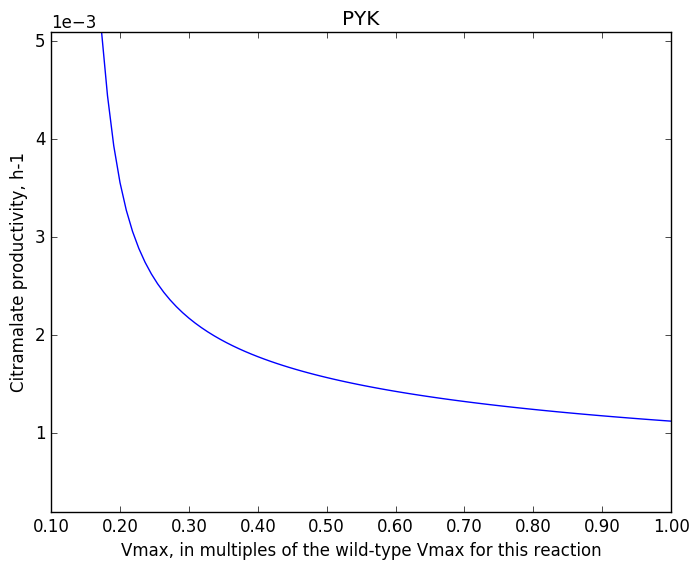
\includegraphics[scale=0.5]{onereacsample}
  \caption{Example of a one-reaction plot: the reaction PYK}
  \label{fig:onereacsample}
\end{figure}

For some reactions, varying $V_{max}$ values had a greater effect on citramalate productivity than others. I quantified this effect based on the data points of the 0.5 -- 2.0 $V_{max}$ plots\footnote{created early in the project, not included in the final results. I only mention them here because I used information from them in later parts of the project} by taking the difference between the maximum and minimum productivities obtained over the range. This method is discussed along with potential alternatives in section~\ref{sec:issues}. Using these difference values, I ordered the reactions into a list, included in appendix~\ref{ap:onereactionlist}, which will be referred throughout this report as the `one-reaction list'.

This identified CITRA\_SYN, GLT, LPD, GROWTH, ATP\_MAINTENANCE, GDH, ATP\_SYN, ACEA, PYK, and ZWF as among the reactions that had the greatest effects. Millard \emph{et al.}~\cite{millard_metabolic_2017} listed CYTBO, ZWF, GDH, GLT, and GROWTH as the reactions found to have the largest shares of flux control. They also exert the strongest controls on concentration. These reactions are followed by LPD, ATP\_MAINTENANCE, ACEA, ATP\_SYN, and PYK.

Exchange reactions (XCH\_ACE, XCH\_GLC, and XCH\_P) had no bearing on productivity as all the data points in their plots could be attributed to noise. Surprisingly, ACS, ACK, and PTA which directly controlled acetyl CoA levels, did not seem to have significant bearings on productivity. As expected, enzymes that have the largest shares of flux control created the plots that demonstrated the greatest changes in citramalate productivity in response to $V_{max}$ variation. However, CYTBO had less effect on productivity as would be expected by this explanation. Although PYK did not exert a lot of control over fluxes as expected by its flux control coefficient, it had a large effect on citramalate productivity. Possibly it was because the citramalate reaction used up pyruvate and because PYK is a control point in glycolysis. Some reactions exhibited inflection points in their plots, as shown in table~\ref{tab:inflection}.

\begin{table}[h]
  \caption{Reactions with inflection points}
  \label{tab:inflection}
  \centering
  \begin{tabular}{lrrl}
    \toprule
    Reaction & $V_{max}$ (mM s\textsuperscript{-1}) & Productivity (h\textsuperscript{-1}) & Type\\
    \midrule
    ATP\_syn & 16.804 & 0.00216 & minimum\\
    & 23.724 & 0.00231 & maximum\\
    CITRA\_SYN & 0.545 & 0.01660 & maximum\\
    CYTBO & 5.124 & 0.00113 & maximum\\
    EDA & 0.014 & 0.00112 & maximum\\
    GDH & 4.569 & 0.00149 & maximum\\
    MQO & 1.597 & 0.00098 & minimum\\
    PFK & 0.145 & 0.00113 & maximum\\
    \bottomrule
  \end{tabular}
\end{table}

In addition, I also extracted a list of reactions arranged by descending order of flux control coefficent (FCC) from the Millard \emph{et al.} paper, and used it alongside the one-reaction list in later parts of the project.

\section{Varying $V_{max}$ values of two reactions at a time}
\label{sec:couples}

Varying $V_{max}$ values of two reactions at a time aimed to identify pairs of reactions that had significant effects on citramalate productivity, and this could be used to identify conditions that optimised citramalate productivity. Ideally, all pairs from the 49 reactions that have $V_{max}$ as a parameter should be investigated. To save computation time and to produce only useful information, I used the eight reactions at the top of the one-reaction list: CITRA\_SYN, GLT, LPD, ATP\_MAINTENANCE, GDH, ATP\_syn, ACEA, and ZWF.

I varied their $V_{max}$ values within 0.1--1.0 $V_{max}$ or 0.1--10.0 $V_{max}$, and plotted the resulting citramalate productivities on heatmaps (see figure~\ref{fig:heatmapsample}). The $V_{max}$ values took 10 values in their ranges, so each heatmap had 100 data points. The horizontal axis indicates the respective $V_{max}$ value of the first reaction in mM s\textsuperscript{-1} and the vertical axis represents the second reaction. Because the wild-type productivity is 0.001122 h\textsuperscript{-1}, I multiplied the citramalate productivity values by 10,000 so that numbers that can be easily conceptualised are displayed on the heatmaps. In figure~\ref{fig:heatmapsample}, when the $V_{max}$ of GLT is 256.76 mM s\textsuperscript{-1} and the $V_{max}$ of ACEA is 1.83 mM s\textsuperscript{-1}, productivity is 0.00848 h\textsuperscript{-1}.

\begin{figure}[hbp]
  \centering
  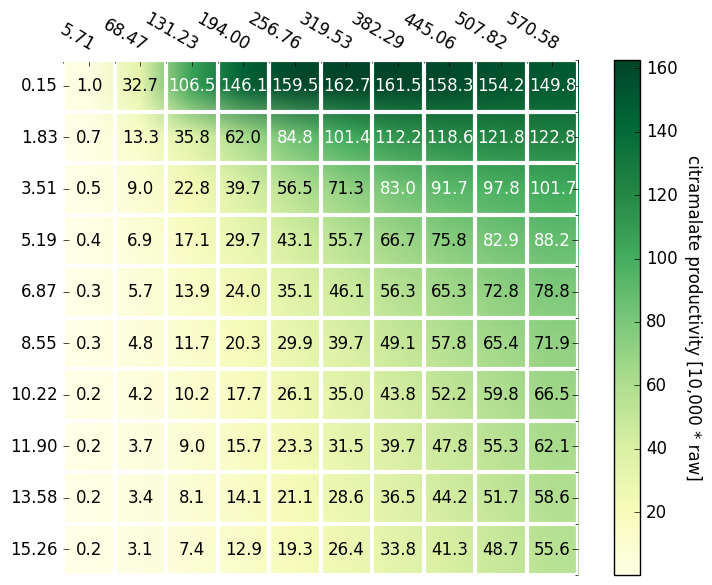
\includegraphics[scale=0.5]{heatmapsample}
  \caption{Example of a heatmap: GLT vs ACEA}
  \label{fig:heatmapsample}
\end{figure}

I also used the reactions with the 10 greatest FCCs to generate heatmaps. The trends seen in most heatmaps suggested simple additive effects, and the heatmaps did not have any additional local maxima or minima, suggesting orthogonality. Plots that involved ATP\_MAINTENANCE exhibited strange behaviour, more evident in higher-resolution heatmaps like figure~\ref{fig:atpmaintenanceheatmap}. This can be attributed to the data between 0.20 and 0.25 $V_{max}$ in ATP\_MAINTENANCE's one-reaction plot (figure~\ref{fig:atpmaintenanceonereac}). Dr J\'ulvez suggested that the model was not configured for such small values of $V_{max}$.

\begin{figure}[hp]
  \centering
  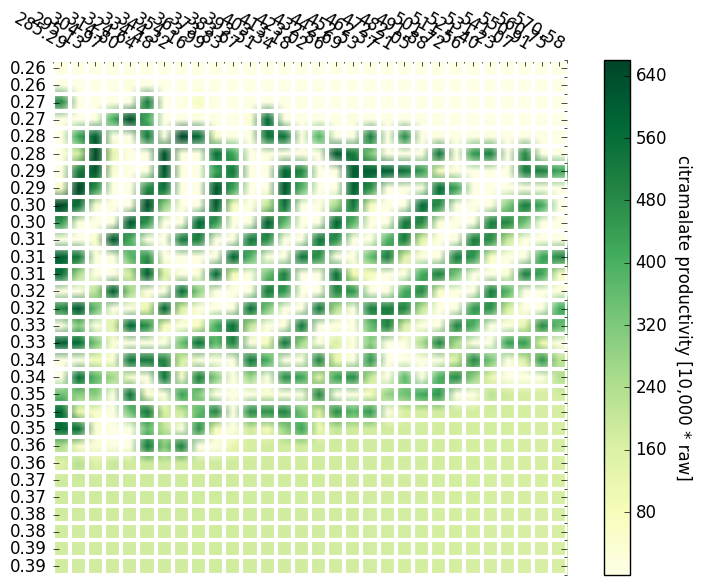
\includegraphics[scale=0.5]{atpmaintenanceheatmap}
  \caption{High-resolution heatmap of GLT vs ATP\_MAINTENANCE}
  \label{fig:atpmaintenanceheatmap}

  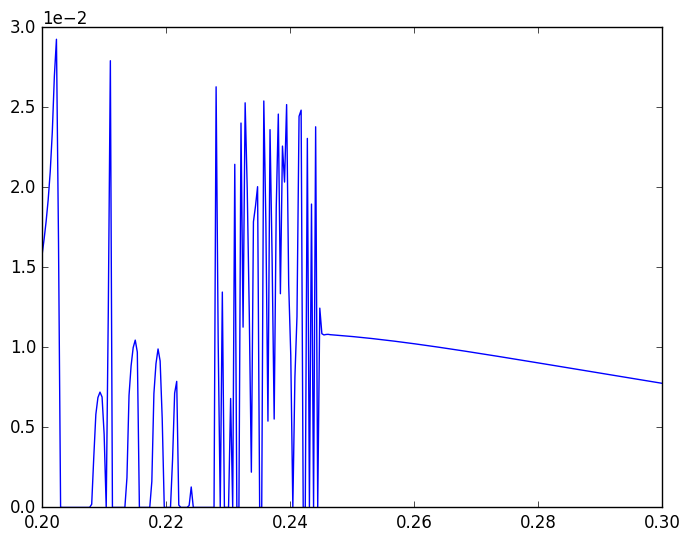
\includegraphics[scale=0.5]{atpmaintenanceonereac}
  \caption{One-reaction plot for ATP\_MAINTENANCE, 300 data points}
  \label{fig:atpmaintenanceonereac}
\end{figure}

\subsection{Steady-state verification}
\label{ssec:steadystate}

The results are only valid if the system has reached steady state. Steady state is achieved if at the end of simulation time, the greatest rate of change of concentration among the species in the system is less than a small threshold value. In other words:

\[
  \max_{X_{i}} \left | \frac{\mathrm{d}[X_{i}]}{\mathrm{d}t} \right | < \epsilon
\]

where X represents a chemical species, and $\epsilon$ is the threshold value. The threshold value was intially set at \num{1.0e-8}, but then adjusted to \num{1.0e-6} following inspection of the heatmaps. For  visualisation, I generated heatmaps with data points replaced by -1 if the system does not reach steady state (figure~\ref{fig:steadystate})

\begin{figure}[hbp]
  \centering
  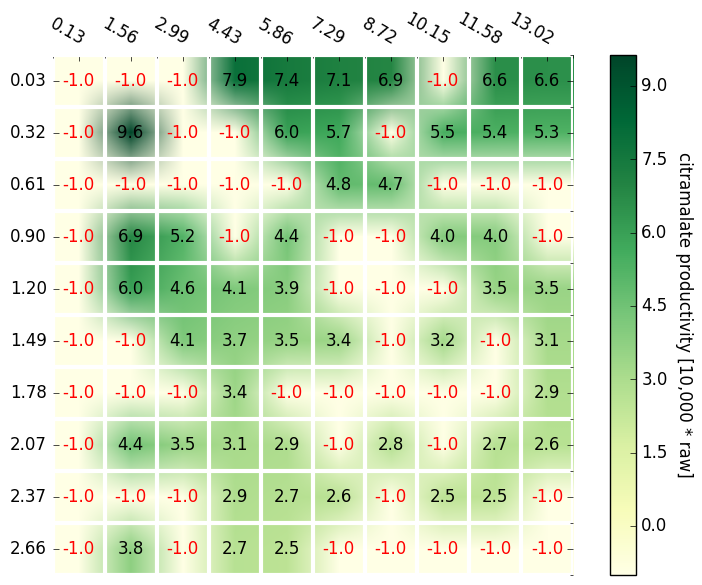
\includegraphics[scale=0.5]{steadystate}
  \caption{Heatmap for ATP\_MAINTENANCE vs ZWF, with threshold set to \num{1.0e-8}}
  \label{fig:steadystate}
\end{figure}

In most cases, ATP, ADP, P, or Hout was responsible for breaking the \num{1.0e-8} threshold. However, their rates stayed at around \num{1.0e-7}. ATP\_MAINTENANCE set at 0.1 $V_{max}$ produced rates on the order of \num{e-1}, and ATP\_syn set at 0.1 $V_{max}$ produced rates on the order of \num{e-2}. With these two reactions, the species responsible for breaking the threshold were BPG and OAA. GDH set at 0.1 $V_{max}$ produced rates on the order of \num{e-3}, with GLCx and GLCp responsible. This was the only situation where GLCx and GLCp concentrations did not reach steady state.

\section{Using differential evolution}
\label{sec:de}

Differential evolution is a genetic algorithm developed by Storn and Price~\cite{storn_differential_1997}. I used the \texttt{rand/1/bin} strategy, adapting code by Mier (2017)~\cite{mier_tutorial_2017, mier_small_2017} to maximise the citramalate productivity while the $V_{max}$ values of multiple reactions in a list were varied simultaneously. Differential evolution includes the following parameters: $F$, the mutation constant or differential weight; $CR$, the recombination constant or crossover probability, $NP$, the population size; and $D$, the number of dimensions, equal to the number of reactions investigated simultaneously. The number of iterations must also be specified.

I used the citramalate productivity calculated after \texttt{roadrunner} simulations as the objective function. Using Mier's parameter values, differential evolution agreed with heatmaps in identifying the $V_{max}$ values that resulted in maximal productivity. Occasionally, it discovered maxima not evident in the heatmaps, owing to the relatively low resolution of the heatmaps. 

\subsection{Finding optimal parameters}
\label{ssec:deoptimise}

I tested how well the suggested differential evolution parameter values quoted by Storn (1996)~\cite{storn_usage_1996} and Pedersen (2010)~\cite{pedersen_good_2010} optimised citramalate productivity. I used reactions in the glycolytic pathway (rationale explained in subsection~\vref{ssec:glycolytic}) and the one-reaction list. Values were chosen based on algorithm run time and how fast convergence was realised. They are presented in table~\vref{tab:deoptimise}.

\begin{table}[htb]
  \caption{Differential evolution optimal parameter search}
  \label{tab:deoptimise}
  \centering
  \begin{tabularx}{\linewidth}{LLLLLLL}
    \toprule
    $F$ & $CR$ & $NP$ & iterations & $D$ & Source\\
    \midrule
    0.8 & 0.7 & 20 & & 2-3 & Mier\\
    0.8 & 0.7 & 20 & 25-40 & 5 & Mier\\
    0.6 & 0.9 & \textless 40 & \textgreater 20 & 5 & Storn\\
    0.6301 & 0.7122 & 17 & 50 & 6-7 & Pedersen (D = 5)\\
    0.6301 & 0.7122 & 17 & 70 & 7 & Pedersen (D = 5)\\
    0.6607 & 0.9426 & 28 & 50 & 7-10 & Pedersen (D = 10, first set), best\\
    0.6702 & 0.2368 & 12 & 100 & 7 & Pedersen (D = 10, second set)\\
    \bottomrule
  \end{tabularx}
\end{table}

\subsection{Optimisation of citramalate production}
\label{ssec:optcitra}

Using the best differential evolution parameters ($F$ = 0.6607, $CR$ = 0.9426, $NP$ = 28, and 50 iterations, as listed in table~\ref{tab:deoptimise}) with the set of seven reactions CITRA\_SYN, GLT, LPD, GDH, ATP\_syn, ACEA, and ZWF, varying $V_{max}$ values over 0.1--10.0 $V_{max}$ yielded optimal $V_{max}$ values as shown in table~\vref{tab:optcitra7} and the citramalate productivity of \num{353.66e-4} h\textsuperscript{-1}. I then changed the $V_{max}$ values of these seven reactions to values expected to maximise citramalate productivity as inferred from the one-reaction plots (section~\ref{sec:onereac}) alone. The resulting productivity was \num{226.96e-4} h\textsuperscript{-1}, lower than the productivity found from differential evolution, confirming the usefulness of the genetic algorithm.

\begin{table}[hp]
  \caption{Optimal $V_{max}$ values, using seven reactions from the one-reaction list}
  \label{tab:optcitra7}
  \centering
  \begin{tabular}{lSl}
    \toprule
    Reaction & \multicolumn{1}{c}{Optimal $V_{max}$} & Remark\\
    \midrule
    CITRA\_SYN & 0.4382 & \\
    GLT & 5.706 & 0.1 $V_{max}$ \\
    LPD & 0.006844 & 0.1 $V_{max}$ \\
    GDH & 3.591 & \\
    ATP\_syn & 10.87 & 0.1 $V_{max}$ \\
    ACEA & 0.1526 & 0.1 $V_{max}$ \\
    ZWF & 0.02658 & 0.1 $V_{max}$\\
    \bottomrule
  \end{tabular}
\end{table}

Furthermore, I tried the same parameters on 10 enzymes and achieved the productivity of \num{405.5e-4} h\textsuperscript{-1} with a set of $V_{max}$ values shown in table~\vref{tab:optcitra10}. However, 10 reactions exhibited slower convergence, as expected by the `curse of dimensionality'. This is a limitation of differential evolution in which the difficulty of finding solutions increases exponentially as dimensions increase.

\begin{table}[hp]
  \caption{Optimal $V_{max}$ values, using ten reactions from the one-reaction list}
  \label{tab:optcitra10}
  \centering
  \begin{tabular}{lSl}
    \toprule
    Reaction & \multicolumn{1}{c}{$V_{max}$ in best solution} & Range\\
    \midrule
    CITRA\_SYN & 1.689 & \\
    GLT & 17.35 & 0.1 $V_{max}$ \\
    LPD & 0.007174 & $\approx$ 0.006844 \\
    GDH & 0.8910 & 0.08666 $\sim$ 0.08910\\
    ATP\_syn & 10.87 & 10.87 $\sim$ 13.01 \\
    ACEA & 0.1826 & 0.1529 $\sim$ 0.01826 \\
    PYK & 0.007472 & $\approx$ 0.007472 \\
    ZWF & 0.02658 & always 0.02658 \\
    NDHII & 10.45 & \\
    MQO & 0.4623 & almost always 0.4623\\
    \bottomrule
  \end{tabular}
\end{table}

I repeated the investigation using the ten enzymes with the greatest FCCs, with results shown in table~\vref{tab:optfcc10}. In this case, the productivity was \num{224.2e-4} h\textsuperscript{-1}. I excluded ATP\_MAINTENANCE because it does not correspond to an enzyme that exists in \emph{E. coli} and because it was not reliable with small values of $V_{max}$, as discussed in section~\ref{sec:onereac}.

\begin{table}[hp]
  \caption{Optimal $V_{max}$ values, using ten reactions with the greatest FCCs}
  \label{tab:optfcc10}
  \centering
  \begin{tabular}{lSl}
    \toprule
    Reaction & \multicolumn{1}{c}{Optimal $V_{max}$}\\
    \midrule
    CYTBO & 3.416 \\
    MQO & 1.849 \\
    MDH & 61.15 \\
    ZWF & 0.1072 \\
    GLT & 378.7 \\
    GDH & 4.485 \\
    ATP\_syn & 43.49 \\
    ACK & 20.15 \\
    ACEA & 0.6189 \\
    EDD & 0.6605\\
    \bottomrule
  \end{tabular}
\end{table}

Using all 41 biologically relevant reactions that have $V_{max}$ as a parameter did not exhibit enough convergence due to the high number of dimensions. However, this produced productivities on the order of \num{200e-4} every time the algorithm was repeated, which was still a significant improvement from wild-type productivity.
\subsection{Glycolytic enzymes}
\label{ssec:glycolytic}

Originally I used differential evolution with the glycolytic enzymes PGI, PFK, FBA, GDH, PGK, GPM, ENO, PYK, and PDH to investigate whether the $V_{max}$ values of all enzymes in a pathway must be increased for an appreciable increase in the overall flux through the pathway, leading to higher productivity. From their experiments on the tryptophan synthesis pathway in yeast, Niederberger \emph{et al.}~\cite{niederberger_strategy_1992} concludes that the fluxes through each enzyme in a linear pathway must all be increased to increase the flux through the pathway. However, Yamamoto \emph{et al.}~\cite{yamamoto_overexpression_2012} show that appreciable increases result after increasing the flux through only one or two enzymes. My results, included in \texttt{kinetic/result/de/gly.txt} support the latter.

I changed the objective to investigating how much adding one reaction as an additional dimension in differential evolution affects productivity. Adding enzymes relatively low on the one-reaction list had little effect on the optimum $V_{max}$ values found earlier, and did not cause large improvements in productivity. This suggested that not all reactions in a network have to be included in differential evolution to produce valid results. The conclusion is beneficial as it reduces computation time needed to optimise citramalate productivity.

\chapter{Enriching the stoichiometric model}
\label{ch:stoich}

The stoichiometric model contains flux bounds -- lower and upper bounds -- for each reaction. These bounds can be specified to provide constraints for flux balance analysis (FBA)\footnote{Orth \emph{et al}~\cite{orth_what_2010} wrote a very good introduction.}. Using linear programming, FBA aims to find an optimal solution for an objective function, subject to constraints on flux values. The objective function can be minimised or maximised, and this can be specified when using \texttt{cobra} to compute the solutions. The lowest and highest possible values of fluxes through each reaction in the kinetic model provides reasonable bounds for the stoichiometric model.

It should be noted that fluxes are in mM s\textsuperscript{-1} in the kinetic model, while they are mmol g\textsubscript{DW}\textsuperscript{-1} h\textsuperscript{-1} in the stoichiometric model. Using the cell volume of \num{1.77e-3} L g\textsubscript{DW}\textsuperscript{-1} as specified in the kinetic model, I worked out that converting units from the kinetic model to the stoichiometric model involves multiplying by 6.372. Because the stoichiometric model does not have information about enzyme kinetics, the values associated with the kinetic model (with kinetic model units) can be used with the structure of the stoichiometric model without any adjustments.

\section{Creating boundaries for flux balance analysis}
\label{sec:bounds}

I varied the $V_{max}$ values of the 49 reactions with $V_{max}$ as a parameter in the kinetic model (with the citramalate synthesis reaction added) to find the the lowest and highest possible values of the fluxes through the 69 reactions in the model. Ideally, all the values should be varied together, but to save computation time, I first varied $V_{max}$ values of one reaction at a time. I did so over the range of 0.1-10.0 $V_{max}$.

Then, I varied the $V_{max}$ values of many reactions at a time using differential evolution, obtaining minimum and maximum values of flux. I used a method similar to that used in section~\ref{sec:de} to obtain the minimum values, specifying the flux through each of the 69 reactions in the kinetic model as the objective function in turn, in place of citramalate productivity. Obtaining the maximum values was a matter of adding a minus sign to the objective function in the script.

First, I included the eight reactions with the greatest flux control coefficients: CYTBO, MQO, MDH, ZWF, GLT, GDH, ATP\_syn, and ACK. The differential evolution parameters used were $F$ = 0.6607, $CR$ = 0.9426, $NP$ = 28, and 5 iterations~\cite{pedersen_good_2010}. I used the $V_{max}$ range of of 0.3--10.0 $V_{max}$ as using $V_{max}$ values less than 0.3 $V_{max}$ tended to produce run time errors in the \texttt{roadrunner} simulation, involving convergence test failures occurring too many times.\footnote{\texttt{RuntimeError: CVODE Error: CV\_CONV\_FAILURE: Convergence test failures occurred too many times (= MXNCF = 10) during one internal timestep or occurred with \textbar{}h\textbar{} = hmin.; In virtual double rr::CVODEIntegrator::integrate(double, double)}} Judging by the behaviour of ATP\_MAINTENANCE, as described in section~\ref{sec:couples}, results were likely unreliable with small $V_{max}$ values, justifying the use of the more restricted range.

With the 41 enzyme-catalysed reactions in the kinetic model with $V_{max}$ as a parameter, I used the differential evolution parameters of $F$ = 0.6876, $CR$ = 0.9784, $NP$ = 48~\cite{pedersen_good_2010}, and five iterations. To avoid convergence test failures, I set the $V_{max}$ range to 0.5--10.0 $V_{max}$.

Bounds generated by including 41 reactions were mostly wider than both bounds generated by including 8 reactions and bounds generated by varying one reaction at a time. In a set of bounds constructed from choosing the best bounds from the three sets, 43 out of 57 lower bounds and 42 out of 57 upper bounds for reactions in the stoichiometric model with equivalents in the kinetic model were from the bounds generated by including 41 reactions.

\section{Mapping reactions in the kinetic model to the stoichiometric model}
\label{sec:mapping}

Previously, an Anargyros who worked in this group produced a mapping table which mapped reactions in the kinetic model to reactions in the stoichiometric model, and included flux bounds. He focused more on mapping so he did not put specific constraints when generating the bounds, and the method by which he generated these values was not documented. I updated the mapping spreadsheet by correcting mistakes and mapping more enzymes. Table~\ref{tab:mapping} presents the mapping changes I made to correct the mistakes.

\begin{table}[htb]
  \label{tab:mapping}
  \caption{Changes to mapping pairs in the mapping table}
  \centering
\begin{tabularx}{\linewidth}{|L|L|L|}
  \hline
  \bfseries Before & \bfseries After & \bfseries Notes\\
  \hline
  Kinetic MDH $\rightarrow$ Stoich MDH2 & Kinetic MDH $\rightarrow$ Stoich MDH, and the reactions are reversed with respect to each other. & Corrected confusion between types of malate dehydrogenases. Re-mapping judged from EC numbers and substrates in the reactions\\
  \hline
  Kinetic XCH\_GLC $\rightarrow$ Stoich GLCtexi & Kinetic XCH\_GLC $\rightarrow$ Stoich GLCtex & Chose a reversible reaction to replace an irreversible one\\
  \hline
  Kinetic XCH\_ACE2 $\rightarrow$ Stoich ACACtex & Kinetic XCH\_ACE2 $\rightarrow$ Stoich ACtex & Corrected a mistake -- it's acetate exchange, not acetoacetate exchange\\
  \hline
\end{tabularx}
\end{table}

Because reactions in the stoichiometric model are not identical to their kinetic counterparts, I devised specific rules to reconcile differences. Stoichiometric model reactions that are identical, reactions that only differ by having small chemical species like \ce{H^+} and \ce{H2O}, reactions that only differ by having \ce{CO2} instead of \ce{HCO3^-}, or reactions that are indicated as irreversible while its equivalent is reversible in the kinetic model have the same lower and upper bounds as their kinetic model counterparts.

For stoichiometric model reactions that are reversed with respect to their kinetic model counterparts, the values obtained from the kinetic model were negated -- i.e.\\ $ \mathrm{Kinetic } (lb, ub) \rightarrow \mathrm{Stoichiometric } (-ub, -lb)$. %overfull hbox quick fix

\begin{figure}[p]
  \centering
  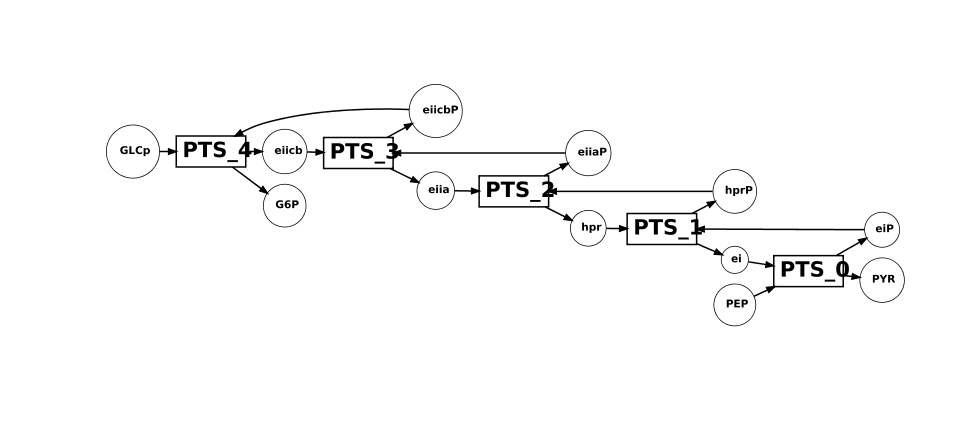
\includegraphics[scale=0.4]{glucoseuptake}
  \caption{Subnetwork for glucose uptake}
  \label{fig:glucoseuptake}
\end{figure}

\begin{figure}[p]
  \centering
  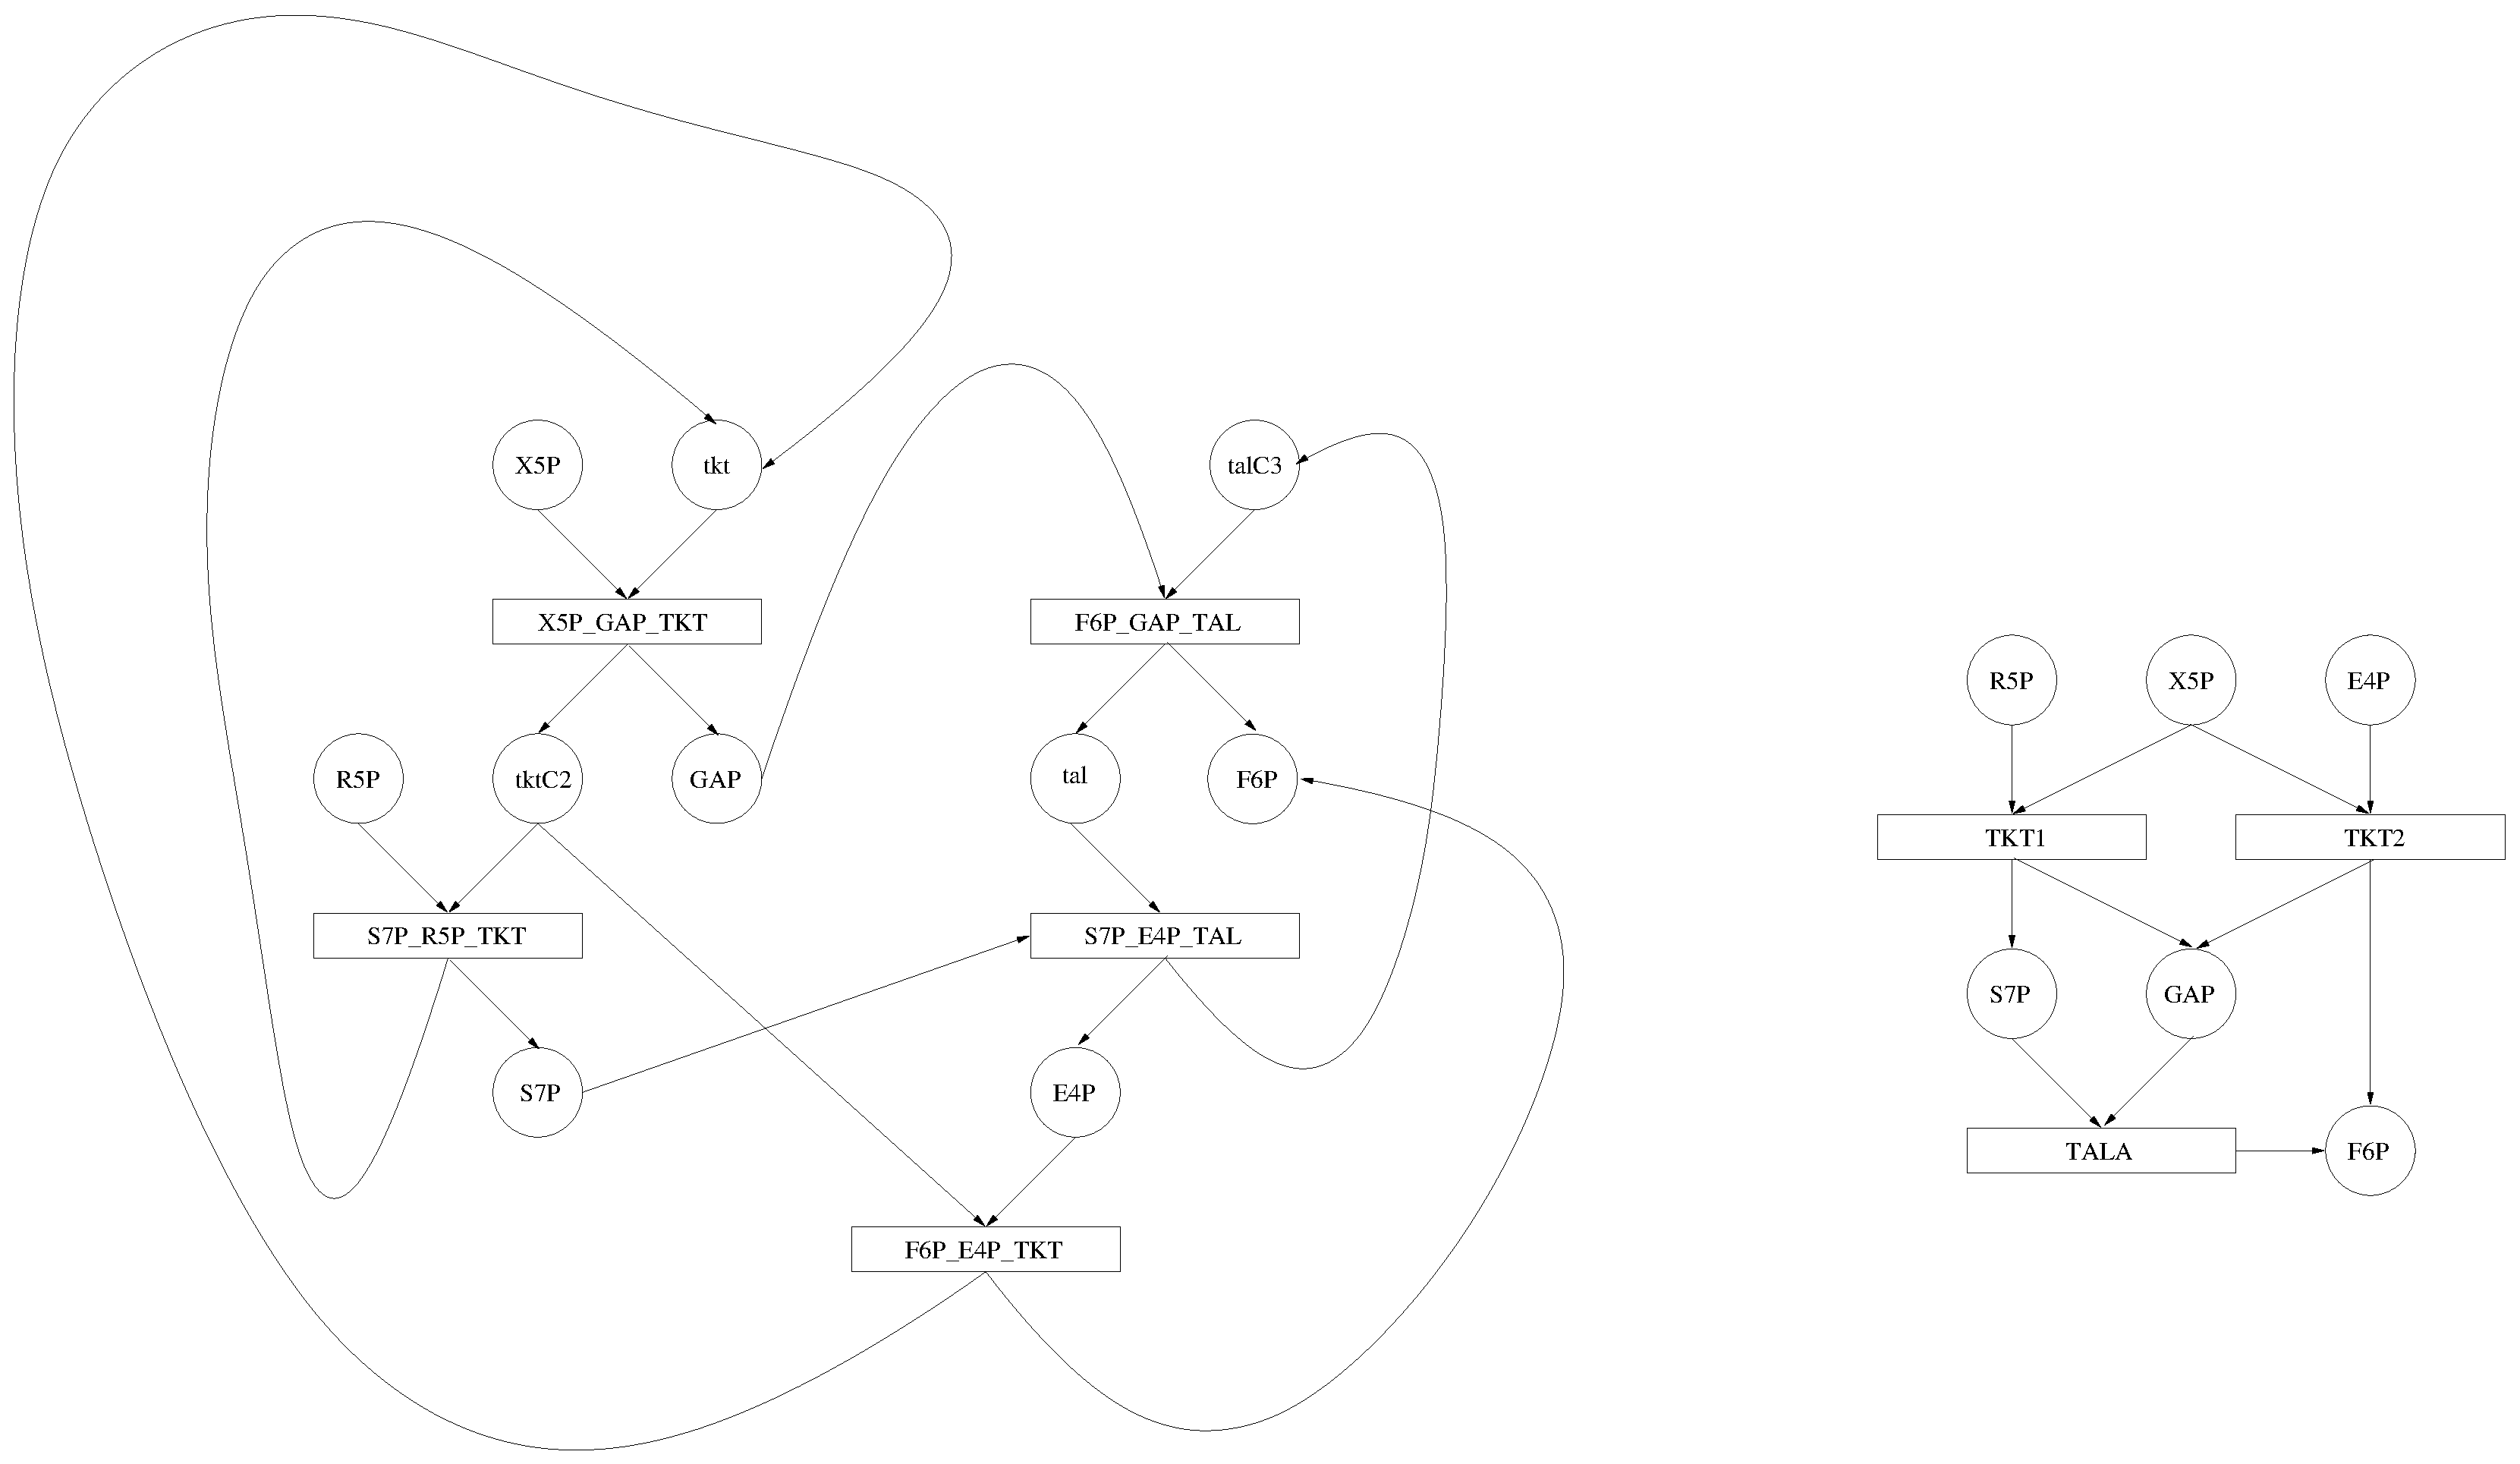
\includegraphics[scale=0.25]{ppp}
  \caption{Subnetwork for part of the pentose phosphate pathway; left - kinetic model, right - stoichiometric model}
  \label{fig:ppp}
\end{figure}

Glucose uptake reactions (PTS\_0, PTS\_1, PTS\_2, PTS\_3, PTS\_4) and the pentose phosphate pathway reactions X5P\-\_GAP\-\_TKT, F6P\-\_E4P\-\_TKT, S7P\-\_R5P\-\_TKT, F6P\-\_GAP\-\_TAL, and S7P\-\_E4P\-\_TAL each form different sub-network structures in the kinetic model compared to the stoichiometric model, and therefore do not allow one-to-one mapping. Figures~\ref{fig:glucoseuptake} and~\vref{fig:ppp} show the structures in the petri net format~\cite{gilbert_unifying_2007, murata_petri_1989}. After investigating the relationship between flux values in both models by conducting simulations, I devised the following solution (applied in \texttt{fba/newmapper.ods}).

\begin{itemize}
\item Force the flux of Stoich TALA to be equal to the flux of Kinetic S7P\_R5P\_TKT.
\item Force the flux of Stoich TKT1 and Stoich TKT2 to be equal to half of the flux of Kinetic RPE.
\item Force the flux of Stoich GLCptspp to be equal to the flux of Stoich GLCtex.
\end{itemize}

These derived from how these relationships between flux values held regardless of the initial conditions.

\section{Investigating glucose uptake}
\label{sec:glucoseuptake}

I then investigated the reactions in both models that relate to glucose uptake in order to evaluate whether there is decoupling between the glucose exchange and glucose uptake reactions. This was done to give insight into the relationship between the extracellular and intracellular concentrations of glucose, which would be useful in determining the effects of a nutrient medium containing glucose on citramalate productivity (discussed in section~\ref{sec:lund}). For clarification on the similar reactions involved, I present how I mapped relevant reactions in the kinetic model to their equivalents in the stoichiometric model in table~\vref{tab:glucoseuptake}.

\begin{table}[hbp]
  \caption{Mapping glucose uptake reactions}
  \label{tab:glucoseuptake}
  \centering
  \begin{tabularx}{\linewidth}{LLL}
    \toprule
    Kinetic model & Stoichiometric model & What it is\\
    \midrule
    GLC\_feed & EX\_glc\_(e) & Glucose feed into the environment, set as 0.23 mM s\textsuperscript{-1} in the kinetic model\\
    XCH\_GLC & GLCtex & Glucose transport from the environment into the periplasm\\
    PTS\_0, PTS\_1, PTS\_2, PTS\_3, PTS\_4 & GLCptspp & Glucose uptake from the periplam into the cytoplasm\\
    \bottomrule
  \end{tabularx}
\end{table}

First, I examined the relationship between glucose feed and the fluxes through the other reactions in the kinetic model. The fluxes through XCH\_GLC and the PTS\_X reactions were always the same. XCH\_GLC was equal to GLC\_feed between 0 and 0.68, otherwise XCH\_GLC stayed at 0.68. With increasing GLC\_feed, GLCx and GLCp concentrations remained very low until GLC\_feed was 0.68, after which they increased linearly as GLC\_feed flux increased. The concentration of G6P increased linearly until GLC\_feed was 0.68, at which it immediately plateaued at 3.19 mM.

\section{Flux balance analysis}
\label{sec:fba}

Using the mapping rules described in section~\ref{sec:mapping}, I prepared bounds for FBA from the kinetic model flux values obtained in section~\ref{sec:bounds}. Setting the objective to maximising to flux through the citramalate flux reaction, I obtained the results in table~\ref{tab:citramalatefluxresults}.

\begin{table}[htbp]
  \caption{FBA results using citramalate flux as the objective function}
  \label{tab:citramalatefluxresults}
  \centering
  \begin{tabular}{lS}
    \toprule
    Bounds & \multicolumn{1}{c}{Solution (mM s\textsuperscript{-1})}\\
    \midrule
    Default & 12.4122\\
    Anargyros's & 0.3067\\
    Varying one reaction at a time & 0.2599\\
    Differential evolution with 8 reactions & 0.1925\\
    Differential evolution with 41 reactions & 0.2922\\
    \bottomrule
  \end{tabular}
\end{table}

I then looped through all 2,585 reactions in the stoichiometric model using each as the objective function. Using the bounds obtained from including 41 reactions in differential evolution, I set the script to evaluate solutions while setting the objective to either maximising or minimising flux. I used the solutions (optimal minmum and optimal maximum values) as an additional set of bounds for another round of FBA, and the solution of 0.2922 mM s\textsuperscript{-1} was returned.

\section{Using information from the Lund medium}
\label{sec:lund}

The patent WO 2015/022496~\cite{eastham_process_2015} describes a fermentation medium on p.79, for \emph{E. coli} BW25113 $\Delta$pflB$\Delta$ldhA transformed with pBAD24-cimA to optimise production of (\emph{R})-citramalic acid:

\begin{tabular}{lSr}
  Glucose & 11.9 & g L\textsuperscript{-1}\\
  \ce{(NH4)2SO4} & 2 & g L\textsuperscript{-1}\\
  \ce{K2HPO4} & 14.6 & g L\textsuperscript{-1}\\
  \ce{NaH2PO4.2H2O} & 3.6 & g L\textsuperscript{-1}\\
  \ce{(NH4)2H} citrate & 0.5 & g L\textsuperscript{-1}\\
  \ce{MgSO4} & 0.24 & g L\textsuperscript{-1}\\
  \ce{CaCl2.2H2O} & 1 & mg L\textsuperscript{-1}\\
  \ce{FeCl3} & 20.06 & mg L\textsuperscript{-1}\\
  \ce{ZnSO4.7H2O} & 0.36 & mg L\textsuperscript{-1}\\
  \ce{CuSO4.5H2O} & 0.32 & mg L\textsuperscript{-1}\\
  \ce{MnSO4.H2O} & 0.30 & mg L\textsuperscript{-1}\\
  \ce{CoCl2.6H2O} & 0.36 & mg L\textsuperscript{-1}\\
  \ce{Na2EDTA.2H2O} & 44.6 & mg L\textsuperscript{-1}
\end{tabular}

This medium is referred to as the `Lund medium' in this project. Each chemical species is present in the following amounts:

\begin{tabular}{lS}
  Species & \multicolumn{1}{c}{Concentration (mM)}\\
  \midrule
  \ce{K^{+}} & 167.6\\
  phosphates & 106.9\\
  glucose & 66.05\\
  \ce{NH4^+} & 34.69\\
  \ce{Na^+} & 23.32\\
  \ce{SO4^{2-}} & 17.13\\
  \ce{Hcitrate} & 2.211\\
  \ce{Mg^{2+}} & 1.994\\
  \ce{Cl^-} & 0.3876\\
  \ce{Fe^{3+}} & 0.1237\\
  EDTA & 0.1198\\
  \ce{Ca^{2+}} & 0.006802\\
  \ce{Mn^{2}+} & 0.001775\\
  \ce{Co^{2}+} & 0.001513\\
  \ce{Cu^{2+}} & 0.001282\\
  \ce{Zn^{2+}} & 0.001252\\
\end{tabular}

To conform to the exchange reactions defined in the stoichiometric model, \ce{HPO4^{2-}} and \ce{H2PO4^-} were merged into one entry representing inorganic phosphates.

I then specifed the maximum rates of exchange of these species by specifying lower bounds for exchange reactions in the stoichiometric model. Exchange reactions for all the above species are present in the stoichiometric model, except for EDTA. I fixed the bound for glucose exchange to -0.23, -0.68, or -10.0, and fixed the bounds for other reactions so that the ratios between the chemical species were consistent. These bounds were added to the set of bounds found in section~\ref{sec:bounds}, in which 41 enzymes were included in differential evolution. With all the glucose exchange bound values described, only the glucose and citrate exchange reactions had non-zero flux values in the optimal solution. When the exchange reactions for the chemical species present in the Lund model were unbounded, glucose exchange was -11.13 and citrate exchange was -1.20, while flux though the citramalate synthesis reaction was found to be 1.1692 mM s\textsuperscript{-1}.

To use the concentrations of the chemical species present in the Lund medium to set the bounds of exchange reactions, rather than using the ratios alone, additional infomation is needed. Given:

\begin{itemize}
\item a concentration of a chemical species $[X_{i}]$
\item the growth rate or dilution rate $\mu$
\item a measured OD\textsubscript{600}, and
\item that an OD\textsubscript{600} of 1 corresponds to an \emph{E. coli} concentration of $Z$, expressed in g\textsubscript{DW} L\textsuperscript{-1} (0.36--0.39 g\textsubscript{DW} L\textsuperscript{-1} in the literature)
\end{itemize}
  
the exchange rate $R$ for that chemical species can be calculated as follows:

\[
  R = \frac{\mu[X_{i}]}{OD_{600} \cdot Z}
\]

However, I was not able to obtain a reliable value for the OD\textsubscript{600} in the experiments described by Orth \emph{et al.}~\cite{orth_comprehensive_2011}, so I was not able to calculate definitive exchange rates (see issues in section~\ref{sec:issues}).

\chapter{Remarks}
\label{ch:remarks}

In this project, I was able to identify reactions in the kinetic model that had relatively large effects on citramalate productivity. Steady-state conditions were achieved in most combinations of $V_{max}$ values used in the project, and situations in which steady-state conditions were not achieved could be attributed to certain reactions acquiring low $V_{max}$ values. I showed that the kinetic model was not reliable with such low values of $V_{max}$. Furthermore, I demonstrated that differential evolution was a viable method to find the best $V_{max}$ values to optimise citramalate productivity, and that only including a small subset of the reactions in the kinetic model was sufficient.

I created an improved method of mapping reactions in the kinetic model to corresponding reactions in the stoichiometric model and assigning bounds for FBA. I also demonstrated that differential evolution could be used to generate useful FBA bounds. Finally, I investigated how the concentrations of chemical species in the Lund medium could be used to set bounds for the exchange reactions in the stoichiometric model.

\section{Issues}
\label{sec:issues}

\urldef\myurl\url{http://sys-bio.github.io/roadrunner/python_docs/api_reference.html?highlight=roadrunner%20roadrunner#the-main-roadrunner-class}

  % defined hyphenation pattens for code in TT to fix overfull hbox
First, \texttt{roadrunner} has a memory leak in \texttt{road\-runner.\-Road\-Runner\-()}. Memory could only be released when the Python program ends. The function was required to run the simulations required to generate almost all the data in the project. \texttt{libsbml\-.write\-SBML\-To\-String\-()} also made a contribution. This function writes a modified SBML file -- in this project, one with modified $V_{max}$ values -- derived from a model object, to a string. \texttt{road\-runner.\-Road\-Runner\-()} then takes the string as an argument to create an object which is used for running simulations. Arguably, it is more logical to pass the model object directly into the simulation, but as of 17 August 2018, the official documentation\footnote{\myurl} for \texttt{libroadrunner} 1.5.1 states that `In future version, we will also support loading directly from a \texttt{libSBML} Document object.'

The memory leak had a large impact on the project as almost all scripts included running simulations on modified kinetic models multiple times in succession. The workaround of writing shell scripts to run and stop the scripts after each round of looping that included running simulations partially alleviated the problem. This method did not work with differential evolution on account of how the algorithm was written. As a result, the number of iterations that could be carried out before Python used up the random access memory in the system was limited, and adequate convergence might not have been realised with high $D$. The `curse of dimensionality', a limitation of differential evolution, exacerbates the problem: with an increasing number of dimensions, the difficulty of finding the optimal solution increases exponentially.

Alternatives to the differential evolution algorithm used in the project exist in the \texttt{scipy} and \texttt{pygmo} modules. These alternatives can use strategies other than \texttt{rand/1/bin} and can carry out self-optimisation of parameters. Furthermore, they can perform dithering on $F$, which was shown to improve convergence~\cite{storn_usage_1996}. However, these alternatives took longer to compute and even exacerbated the memory leak problem, using up more memory for each iteration, presumably because they called the objective function more times. As they are black-box optimisation methods, I was unable to probe into the problem or improve on the algorithms.

Fortunately, the \texttt{cobra} module used to manipulate the stoichiometric model and FBA does not have memory leaks.

Next, I address preparing lists of reactions used in generating heatmaps and in differential evolution. The method I used to quantify the effect that varying $V_{max}$ of each reaction had on citramalate productivity as described in section~\ref{sec:onereac} had no real statistical basis (it was a quick-and-dirty method). Regression did not appear to be informative. Any method that uses the data points I generated, however, would have to rationalise using a specific range of $V_{max}$ values, as the ranges in use are arbitrary. Using the flux control coefficients was an alternative, and I generated data accordingly, but the reactions were sorted by how much control they had over the network as a whole, and not by control over the citramalate synthesis reaction.

Additionally, generating one-reaction plots\footnote{included in the result directories} (section~\ref{sec:onereac}) using flux through the citramalate synthesis reaction and growth as objective functions, in place of citramalate productivity called into question the validity of using flux through the citramalate synthesis reaction as a proxy for citramalate productivity in FBA. The shape of the plots of flux through citramalate synthesis (figure~\vref{fig:issues_citraflux} provides an example) differed a lot from that of citramalate productivity, and growth contributed more to the shape of the plots of citramalate productivity (figure~\vref{fig:issues_igrowth} shows such a plot, which can be compared to figure~\vref{fig:onereacsample}). I investigated the use of citramalate productivity as the objective function in FBA, but \texttt{cobra} was limited to linear functions. As citramalate productivity is expressed as the product of two functions that exist in the stoichiometric model, other packages such as CPLEX or Gurobi must be used. However, both are proprietary, though Gurobi offers a free licence for universities.

\begin{figure}[htbp]
  \centering
  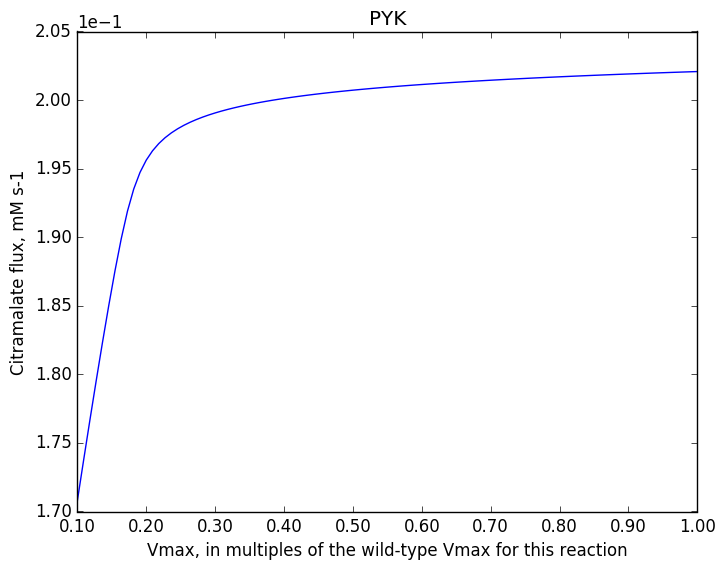
\includegraphics[scale=0.4]{issues_citraflux}
  \caption{Relationship between PYK $V_{max}$ and flux through citramalate synthesis reaction}
  \label{fig:issues_citraflux}
\end{figure}

\begin{figure}[htbp]
  \centering
  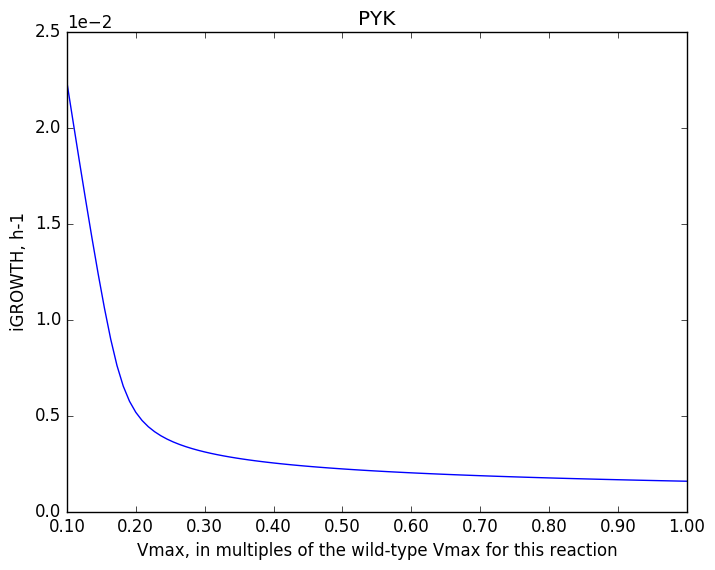
\includegraphics[scale=0.4]{issues_igrowth}
  \caption{Relationship between PYK $V_{max}$ and $\mathrm{iGROWTH}'$. iGROWTH is a species created to model growth in the kinetic model.}
  \label{fig:issues_igrowth}
\end{figure}

I based mapping reactions in the kinetic model to their equivalents in the stoichiometric model (section~\ref{sec:mapping}) on observations from running simulations rather than theoretical knowledge behind the model networks, and the validity of this method is yet to be assessed. However, I observed that switching from Anargyros's more limited treatment of the glucose uptake and pentose phosphate pathway reactions to the method I used did not cause a significant change to the optimal citramalate productivity found by FBA.

Finally, there were issues with working out FBA bounds from the composition of the Lund medium (section~\ref{sec:lund}), which involved translating the concentration of a chemical species into a flux value for the corresponding exchange reaction. This was mainly due to the lack of a definitive OD\textsubscript{600} value for \emph{E. coli} in the stoichiometric model, as Orth \emph{et al.}~\cite{orth_comprehensive_2011} did not specify it. Complicating the issue, a study by Kavvas \emph{et al.}~\cite{kavvas_updated_2018} includes variations of a stoichiometric model for \emph{Mycobacterium tuberculosis} that had different bounds for exchange reactions according to differing media conditions, but the bounds seem to be arbitrary round numbers and do not reflect the ratios between the concentrations of the chemical species in the media. Even if appropriate bounds could be worked out, the observations resulting from unbounding exchange reactions as described in section~\ref{sec:lund} called into question how useful they would be.

\section{Future direction and suggestions}
\label{sec:future}

Improving or building up on this project may include some of the following:

\begin{itemize}
\item Use a simulator apart from \texttt{roadrunner} that does not have a memory leak
\item Use standard deviations to quantify the effect varying $V_{max}$ values of each reaction in the kinetic model has on citramalate productivity
\item Develop a method to investigate whether there are synergistic effects between reactions
\item Investigate alternatives to \texttt{scipy} and \texttt{pygmo} for the implementation of a differential evolution algorithm, and investigating optimal parameter searches -- the fuzzy algorithm described by Liu and Lampinen~\cite{liu_fuzzy_2005} may be an option
\item Use other genetic algorithms apart from differential evolution
\item Use more than five iterations in differential evolution to generate bounds for FBA
\item Investigate the theoretical basis behind mapping between the kinetic and stoichiometric models
  \item Use CPLEX, Gurobi, or other packages to perform FBA using citramalate productivity as the objective function in place of flux through the citramalate synthesis reaction.
\end{itemize}
  
\section{Notes about files}
\label{sec:files}

The files included alongside this report include text files, images, spreadsheets, and Python scripts. The text files mainly contain information about the models, such as wild-type conditions, and results from various parts of the project. The images include the one-reaction plots and heatmaps. Important spreadsheets include an improved version of Anargyros's mapping spreadsheet and one to convert the minimum and maximum fluxes in the kinetic model to corresponding fluxes to be applied in FBA. Finally, the Python scripts were written to manipulate the two models, generate the images, and generate the data in the project. All files are version-controlled by Git.

% remove this paragraph later
These files are in a version-controlled directory and in a \emph{private} GitHub repository owned by \url{https://github.com/arinwongprommoon/}, which only I have access to.

\appendix
\chapter*{Appendix}
\addcontentsline{toc}{chapter}{Appendix}
\renewcommand{\thesection}{\Alph{section}}

\section{Reactions in the kinetic model}
\label{ap:kineticreactionlist}

This is a list of the 68 reactions in the kinetic model with their wild-type $V_{max}$ values as specified in the SBML file. 49 reactions have $V_{max}$ as a parameter.

\begin{longtable}{lS}
  \toprule
  Reaction & \multicolumn{1}{c}{Wild-type $V_{max}$ (mM s\textsuperscript{-1})}\\
  \midrule
  ACEA & 1.52595\\
ACEB & 0.352769\\
ACEK\_1 & \multicolumn{1}{c}{None}\\
ACEK\_2 & \multicolumn{1}{c}{None}\\
ACK & 7.23\\
ACN\_1 & 9.72413\\
ACN\_2 & 9.86571\\
ACS & 7.3\\
ADK & \multicolumn{1}{c}{None}\\
ATP\_MAINTENANCE & 1.30166\\
ATP\_syn & 108.733\\
CYA & \multicolumn{1}{c}{None}\\
CYTBO & 8.54045\\
DOS & \multicolumn{1}{c}{None}\\
EDA & 0.0775241\\
EDD & 0.111359\\
ENO & 11.7189\\
F6P\_E4P\_TKT & \multicolumn{1}{c}{None}\\
F6P\_GAP\_TAL & \multicolumn{1}{c}{None}\\
FBA & 21.6978\\
FBP & 0.215583\\
FUMA & 53.3414\\
GDH & 8.66573\\
GL6P\_HYDROLYSIS & \multicolumn{1}{c}{None}\\
GLC\_feed & \multicolumn{1}{c}{None}\\
GLT & 57.0584\\
GND & 4.08105\\
GPM & 10.9934\\
GROWTH & 9.74137\\
ICD & \multicolumn{1}{c}{None}\\
LPD & 0.0684413\\
MAD & 6.64269\\
MDH & 6.11492\\
MQO & 4.62283\\
NADH\_req & 23.0735\\
NDHII & 30.8306\\
PCK & 8.08777\\
PDH & 961.706\\
PFK & 0.185253\\
PGI & 2.32456\\
PGK & 16.1089\\
PGL & 11.5967\\
PIT & 7.146\\
PNT\_req & \multicolumn{1}{c}{None}\\
PPC & 21.439\\
PPS & 0.0163772\\
PTA & 2.7\\
PTS\_0 & \multicolumn{1}{c}{None}\\
PTS\_1 & \multicolumn{1}{c}{None}\\
PTS\_2 & \multicolumn{1}{c}{None}\\
PTS\_3 & \multicolumn{1}{c}{None}\\
PTS\_4 & \multicolumn{1}{c}{None}\\
PYK & 0.74716\\
RPE & 6.00103\\
RPI & 8.0\\
S7P\_E4P\_TAL & \multicolumn{1}{c}{None}\\
S7P\_R5P\_TKT & \multicolumn{1}{c}{None}\\
SDH & 1.56184\\
SK & 76.8163\\
SQR & 3.41617\\
TPI & 24.1843\\
X5P\_GAP\_TKT & \multicolumn{1}{c}{None}\\
XCH\_ACE1 & 100.0\\
XCH\_ACE2 & 100.0\\
XCH\_GLC & 100.0\\
XCH\_P & 100.0\\
ZWF & 0.2658\\
\_ACE\_OUT & \multicolumn{1}{c}{None}\\
\bottomrule
\end{longtable}

Of these, 41 correspond to real enzymes in \emph{E. coli}: ACEA, ACEB, ACK, ACN\_1, ACN\_2, ACS, ATP\_syn, CITRA\_SYN, CYTBO, EDA, EDD, ENO, FBA, FBP, FUMA, GDH, GLT, GND, GPM, LPD, MAD, MDH, MQO, PCK, PDH, PFK, PGI, PGK, PGL, PIT, PPC, PPS, PTA, PYK, RPE, RPI, SDH, SK, SQR, TPI, and ZWF.

\section{One-reaction list}
\label{ap:onereactionlist}

Here is the list of kinetic model reactions ordered by effect on citramalate productivity, as quantified by the method described in section~\ref{sec:onereac}. This list is termed the `one-reaction list' in this report.
\begin{longtable}{lS}
  \toprule
  Reaction & \multicolumn{1}{c}{Difference}\\
  \midrule
CITRA\_SYN & 0.0047592827\\
GLT & 0.0028143645\\
LPD & 0.0024355991\\
GROWTH & 0.0015196535\\
ATP\_MAINTENANCE & 0.0013313081\\
GDH & 0.0009114522\\
ATP\_syn & 0.0007611072\\
ACEA & 0.0007511846\\
PYK & 0.0007372515\\
ZWF & 0.0003202479\\
NDHII & 0.0002585753\\
MQO & 0.0002267894\\
NADH\_req & 0.0002253453\\
MDH & 0.0002253183\\
MAD & 0.000194721\\
PGI & 0.0001198466\\
PCK & 0.0001030438\\
PPC & 9.98662735514203E-05\\
ACEB & 7.90308554654898E-05\\
PDH & 7.25091053451472E-05\\
ENO & 0.000052497\\
CYTBO & 4.01304504630247E-05\\
PFK & 0.000029278\\
SDH & 2.34810929815527E-05\\
GPM & 0.000017908\\
RPI & 1.57468888476676E-05\\
RPE & 1.17187158724425E-05\\
GND & 7.7970772124512E-06\\
FBA & 5.78669223682236E-06\\
PIT & 4.2598627200143E-06\\
XCH\_GLC & 2.30450409889268E-06\\
EDD & 1.45414534944354E-06\\
TPI & 1.13784049543585E-06\\
ACK & 5.9384816856003E-07\\
SQR & 2.76393130356403E-07\\
ACN\_1 & 0.000000163\\
ACN\_2 & 1.34302723317709E-07\\
PGL & 1.18091121640955E-07\\
EDA & 1.13285023008386E-07\\
FBP & 6.4369739164339E-08\\
PTA & 0.000000059\\
PPS & 3.50591144481546E-08\\
FUMA & 1.57341325584745E-08\\
PGK & 1.23830399983461E-08\\
ACS & 3.41921927208243E-09\\
SK & 2.53497706831883E-09\\
XCH\_ACE1 & 3.6139094993469E-10\\
XCH\_P & 1.30011316599662E-10\\
XCH\_ACE2 & 1.15399255906298E-10\\
\bottomrule
\end{longtable}

\section{Synergistic effects between reactions in the kinetic model}
\label{ap:synergistic}

I investigated whether there were synergistic effects between reactions by investigating reactions adjacent to each other, starting from the glycolytic pathway. No effects were observed for PGI and PFK, and a slight synergistic effect was observed for GPM and ENO. Between FBA and GDH, FBA exerts too little effect for the results to be conclusive. In contrast, ACEA and ACEB exhibit \emph{antagonistic} effects, and LPD and GDH, a pair of enzymes far apart from each other in the network seem to have a synergistic effect. Whether there were synergistic effects between reactions remains inconclusive. My investigations are in \texttt{kinetic/result/couples/Adjacent/Adjacent.txt}.

\printbibliography

\end{document}
